\documentclass{sig-alternate-05-2015}
\usepackage[utf8]{inputenc}
\usepackage[english, francais]{babel}
\usepackage{microtype}
\usepackage{xspace}
\usepackage{amsfonts}
\usepackage{amssymb}
\usepackage{mathtools}
\usepackage{xcolor}
\usepackage{paralist}
\usepackage{booktabs}
\usepackage{wrapfig}
\usepackage{subfigure}
\usepackage{csquotes}
\usepackage{tikz}
\usepackage[pdfborder={0 0 0}, pdfpagelabels=false]{hyperref}
\usetikzlibrary{matrix,shapes.multipart, arrows, shapes.geometric,fit,scopes}
\tikzset{
  >= latex,
  el/.style={ellipse, draw, text width=8em, align=center},
  rs/.style={rectangle split, draw, rectangle split parts=#1},
  ou/.style={draw, inner xsep=1em, inner ysep=1ex, fit=#1}
}
\definecolor{marron}{rgb}{0.8,0.6,0.4}
\newcommand{\lamine}[1]{\textbf{[Lamine: {\textcolor{red}{#1}}]}}
\newcommand{\laure}[1]{\textbf{[Laure: \textcolor{marron}{#1}]}}
\newcommand{\tbd}[1]{\textbf{[TODO: \textcolor{blue}{#1}]}}
\newcommand{\qset}{\ensuremath{\mathcal{Q}}}
\newcommand{\query}{\ensuremath{\mathit{q}}}
\newcommand{\fact}[1]{\ensuremath{\mathit{f}_{#1}}}
\newcommand{\e}[1]{\ensuremath{\mathit{e_{#1}}}}
\newcommand{\claim}[1]{\ensuremath{\mathit{c_{#1}}}}
\newcommand{\claimset}{\ensuremath{\mathcal{C}}}
\newcommand{\rel}[1]{\ensuremath{\mathit{r}_{#1}}}
\newcommand{\source}[1]{\ensuremath{\mathit{s}_{#1}}}
\newcommand{\sset}[1]{\ensuremath{\mathcal{S}_{#1}}}
\newcommand{\TRUE}{\ensuremath{\mathsf{true}}}
\newcommand{\FALSE}{\ensuremath{\mathsf{false}}}


\begin{document}
\conferenceinfo{}{}

\title{Cross-Modal Truth Discovery for Detecting and Corroborating Spatio-Temporal Events in the City}

\numberofauthors{1} 
\author{
\alignauthor
***\\
       \affaddr{Qatar Computing Research Institute}\\
       \affaddr{Tornado Tower, West Bay}\\
       \affaddr{Doha, Qatar}\\
       \email{\{*,*,*\}@qf.org.qa}
}


\maketitle

\begin{abstract}

\end{abstract}

% A category with the (minimum) three required fields
%\category{H.4}{Information Systems Applications}{Miscellaneous}
%A category including the fourth, optional field follows...
%\category{D.2.8}{Software Engineering}{Metrics}[complexity measures, performance measures]

%\terms{Theory}

%\keywords{ACM proceedings, \LaTeX, text tagging}

% Introduction
\section{Introduction}

In recent years, vast amounts of volunteered information have been posted through social media  and Web platforms. Such platforms have sparked an exponential growth of user-generated content in various formats and modalities mixing images, videos, texts, and structured data.  Citizens around the world actively capture own observations of events they may (or may not) witness and make them publicly available on the Web. 
Information about places of interest, events, traffic jams, aggressions are examples of this user-generated content. 
Usually the content consists of a multimedia content with an incomplete description of the place, time, phenomenon or event  eventually with metadata collected by technical devices, e.g., camera type in Flickr images, EXIF.


Evaluating the veracity of such information coming both from volunteering observers or  Web news media is a challenging problem due to many reasons. First, information may be uncertain, incomplete and decorrelated in time and place from the considered real-world event; textual description, keywords or hashtags may be missing/incomplete or ambiguous; conflicting information may be reported by non reliable observers; the duration of some real-world events may be so short that no or very few observers actually witnessed them; not only some events may not be reported but also some observations may not be `linkable' to any of the known events.  Practical settings are far from the best case scenario where many observations have accurate georeferences and timestamps, and  complete descriptions that enable their mapping to one single real-world event with no ambiguity and no conflict.  

To overcome these problems, various methods have been recently proposed to discover
the true value from those provided by a large number of conflicting data sources.  These solutions extend
vote counting strategy with probabilistic inference and Maximum A Posterior (MAP) estimation via Expectation-Maximization and compute iteratively
the accuracy of the sources claiming some data as a function of the confidence of the data they claims (see \cite{} for a complete survey of the current
approaches).

However, current truth discovery methods --mainly applied to structured data extracted from texts-- can not be straighforwardly applied to spatio-temporal and cross-modal data. 
Moreover, they  suffer from data spasity problem also called long-tail phenomenon where very few sources actually report information about all the events whereas the majority of sources report information about very few events.


At a city-scale, local events occuring in urban spaces can be detected using various sources of data: {\it (i)} from social media and social networks 
(e.g., with  Instagram, Filckr, Twitter data), {\it (ii)} from traffic sensors and other monitoring devices operating all over the city (e.g., air pollution, bluetooth sensors), and {\it (iii)} from the blogosphere and Web news. This paper is a first attempt to leverage data cross-modality to infer the truth of  real-world events' occurence and to propagate replacement labels for missing or uncertain information.


 %At a macro-scale, GDELT event database records over 300 categories of physical activities around the world, from riots and protests to peace appeals and diplomatic exchanges, georeferenced to the city or mountaintop, across the entire planet dating back to January 1, 1979 and updated daily.

 

 In summary, this paper makes the following contributions:
 \begin{enumerate}
\item We propose to address the truth discovery problem in the context of cross-modal data for detecting and corroborating of spatio-temporal events.
\item We propose an unsupervised  probabilistic approach  which models the truth of observations and reports related to spatial events and the reliability of the observers. 
\item We develop an efficient optimization algorithm for model inference based on gradient descent and we show that our approach converges faster than EM-based methods with better quality performances.
 \end{enumerate}

The remainder of this paper is organized as follows. We formalize the problem in Section 2.  
We then introduce our proposed model and develop the optimization algorithm in Section 3. 
Experimental setup and results are presented in Section 4. 
Related work is discussed in Section 5. Finally, we conclude the paper in Section 6.

\section{Problem Definition}

We formally define the cross-modal truth discovery problem in this section.
Consider a scenario where a group of users report a specific type of spatio-temporal events (e.g., traffic jam, accident). A user $u$
makes an observation $o$ at time $t$. Each observation $o=(u,l,t,d,c)$ contains the user ID $u$, the location $l$ of the event (e.g., by GPS), the time $t$ of the observation, and the description of the event. The description is a list of  text, keywords or hashtags and  a set of modal features characterizing the content $c$. 

For example, the image  in Fig. 1 posted on Flickr is the content of one observation made by user $Phic$ on Oct. 30, 2013,  around 2 pm, related to traffic at the intersection of Markhiya and Al Bidda roads in Doha, Qatar. This observation is  encoded as: \\
$('Phic', gpslong,gpslat, dateformat,text, imageBLOB )$  to complete

%-----------------------------------
\begin{figure}[t]
 \centerline{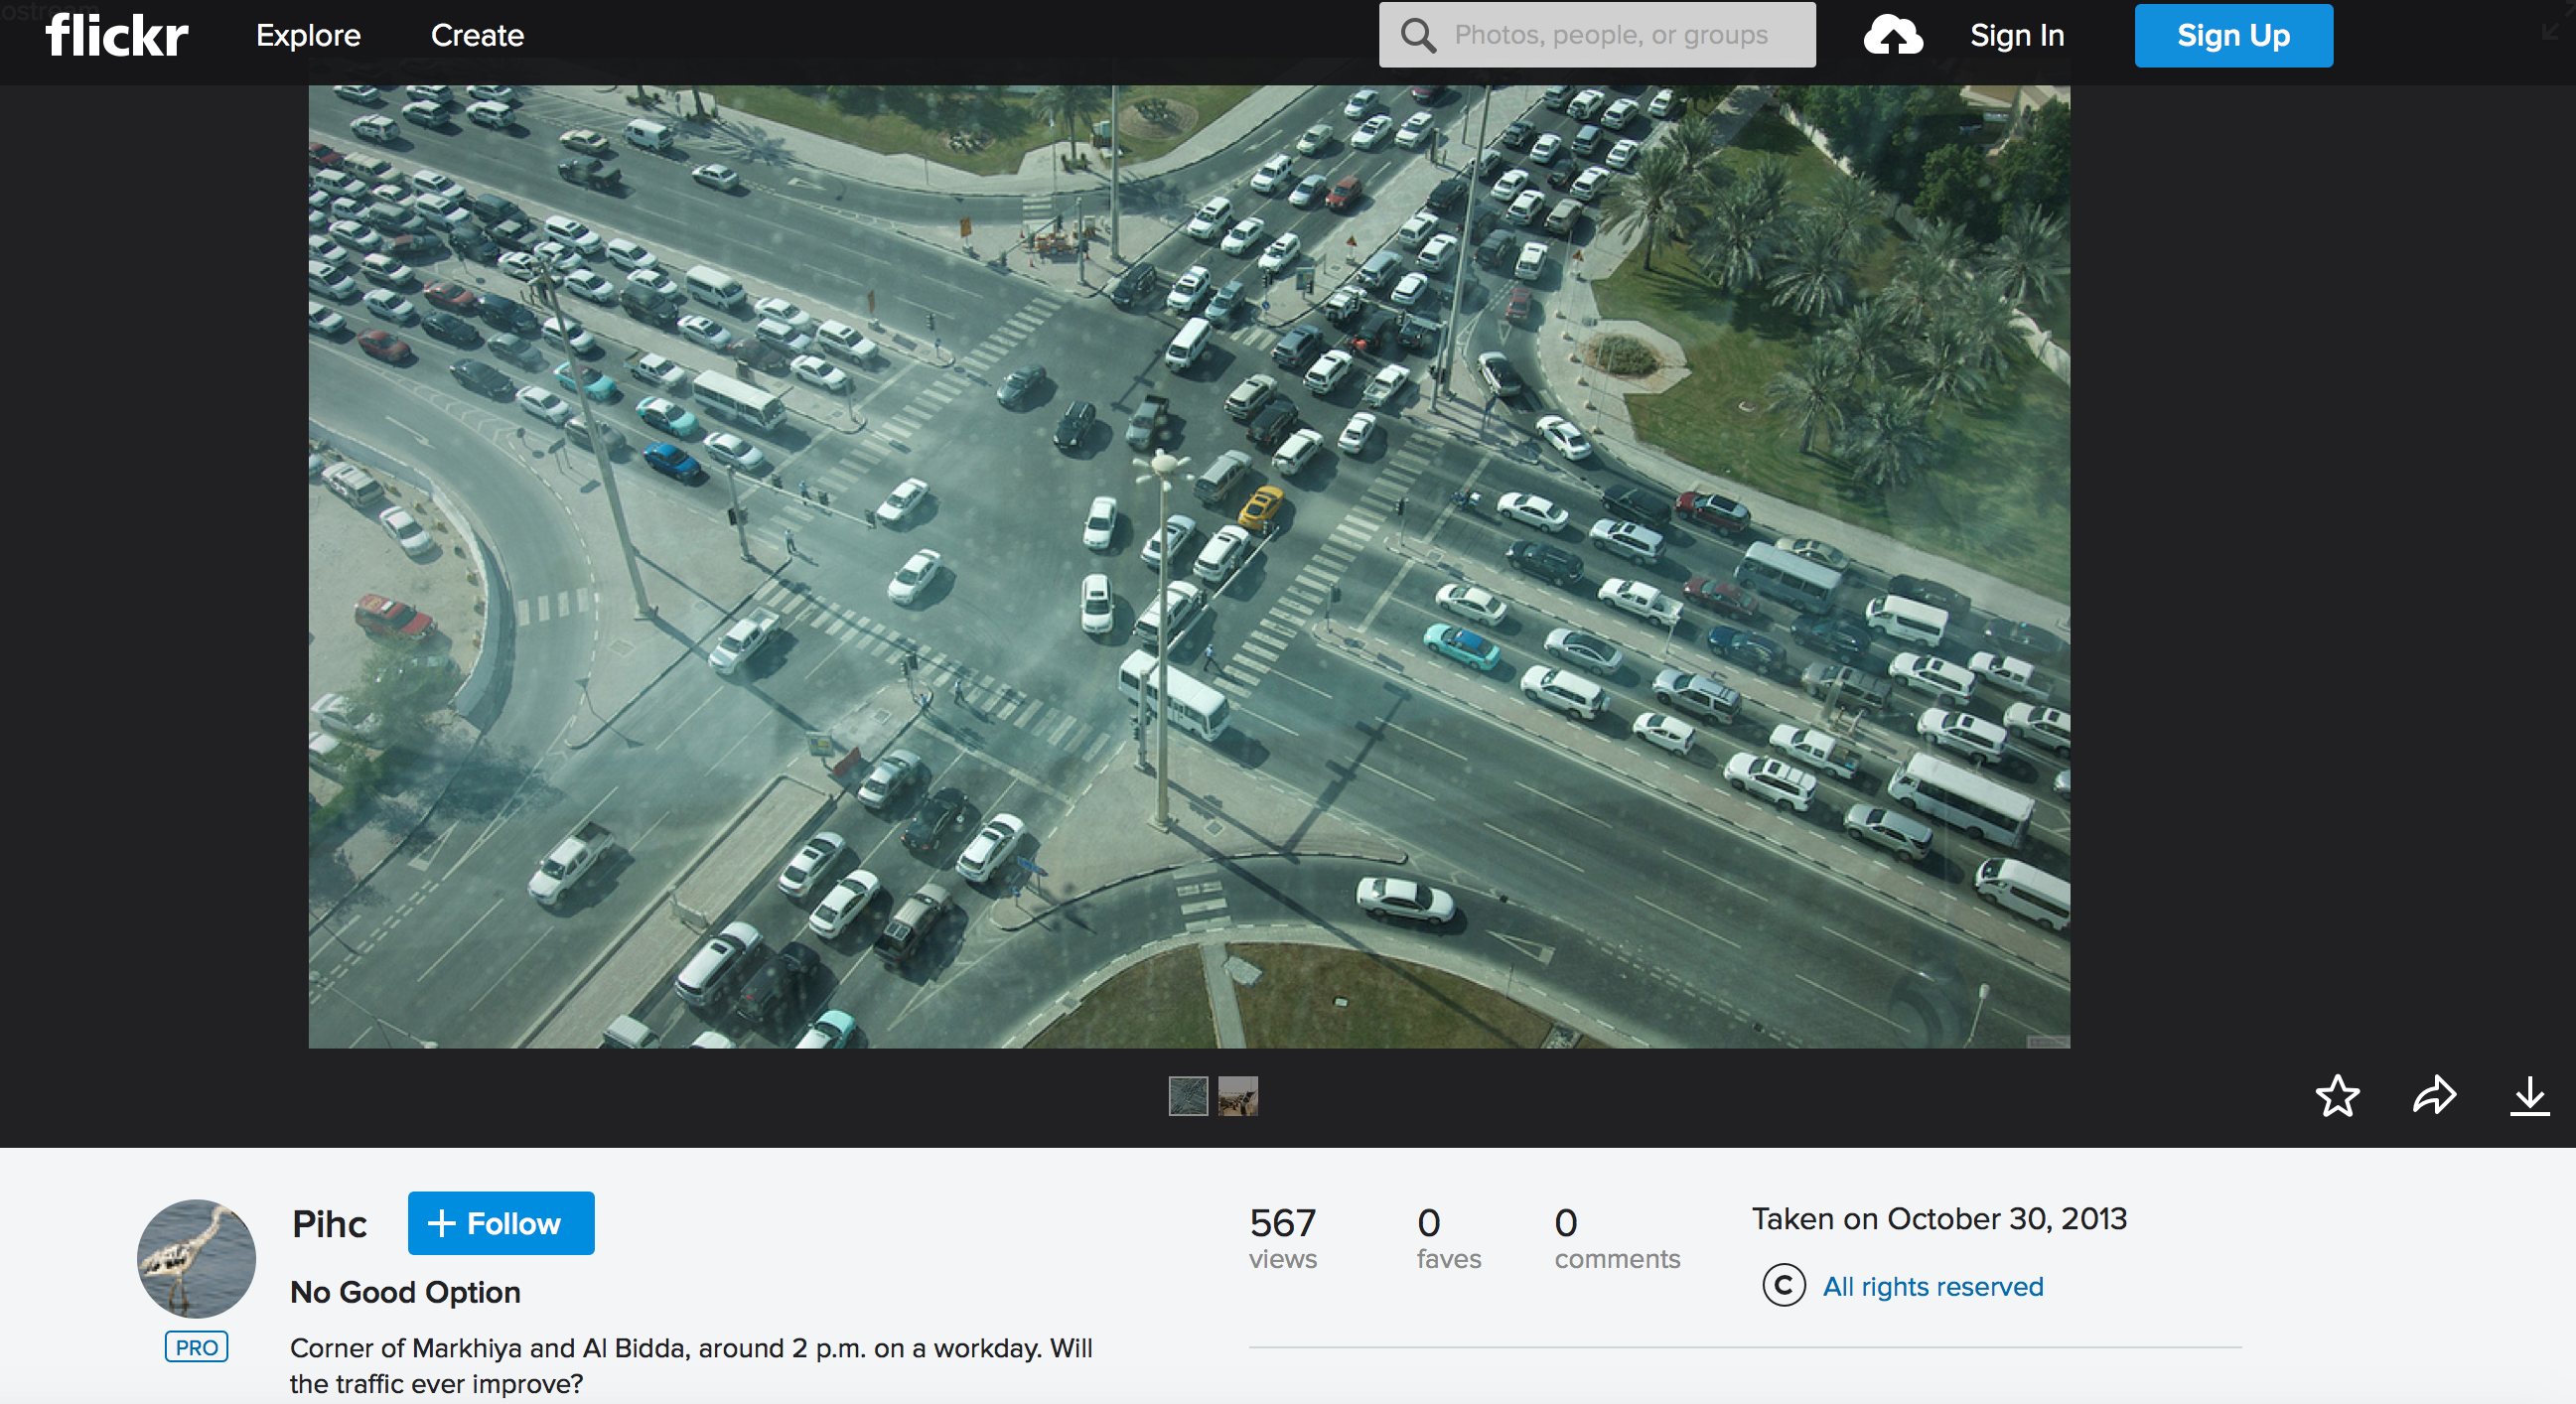
\includegraphics[scale=.45,width=.45\textwidth]{fig-example.png}}
\caption{ Example of observation}
\label{fig1}
\end{figure}
%-----------------------------------

We consider the set of observations collected within a certain time window $\mathcal{T}$ and a spatial
region of interest $\mathcal{S}$ such as:
$$ \mathcal{O}=\{ o \mid o.t \in\mathcal{T}, o.l \in\mathcal{S} \}.$$

  Given $ \mathcal{O} $, the problem we address is first to group together the observations that are most likely referring to the same real-world event (blocking/linking). Second, among the candidate observations linked to a given event, our goal is to infer the most accurate time, location, and description of the event.


\section{Optimization Algorithm}
\section{Related Work}
\section{Conclusion}


% References
%\cite{*}

\bibliographystyle{plain}
\small\bibliography{references}
\end{document}
